\newpage
\section{Технический отчет по практике}

\subsection{Постановка задачи}

С использованием искуственной нейронной сети (ИНС) Fuzzy ART реализовать ПМО обеспечения, позволяющее классифицировать символы русского алфавита.

\subsection{Описание парадигмы Fuzzy ART}


Нейронные сети адаптивной резонансной теории (Adaptive Resonance Theory = ART) или ART-сети образуют целый класс различных нейросетей, предложенных Карпентером (Carpenter) и Гроссбергом (Grossberg) (Бостонский университет, 1987-1991).

В реальной практике часто данные, используемые для обучения или самообучения сети, не стабильны. В этом случае классические нейронные сети не позволят получить требуемого результата.

При анализе систем классификации возникают противоречивые требования или свойства нейросети. С одной стороны очень важно, чтобы она была способна выявлять (обнаруживать) образы новых классов, ранее не представленных сети. Это свойство пластичности. С другой же стороны изученные классы образов должны сохраняться – свойство устойчивости работы нейросетей. Эти два свойства – пластичности и стабильности в известной мере противоречивы – дилемма пластичности-стабильности. Сети ART были разработаны для разрешения этой дилеммы, а именно: для установления новых ассоциаций (классов) нейронной сетью без забывания старых ассоциаций (классов). Семейство ART-сетей включает следующие сети:
\begin{itemize} \compact
	\item ART-1: для бинарных входных векторов, когда признаки распознаваемых образов принимают два значения 1 или 0;
	\item ART-2: расширение ART-1-сетей на непрерывные входные векторы;
	\item ART-2a: оптимальная версия ART-2-сетей, отличающаяся повышенной скоростью сходимости;
	\item ART-3: моделирование временных и химических процессов (биологических механизмов) на базе ART-2;
	\item ARTMAP: комбинация двух ART-сетей (например, ART-1 и ART-2);
	\item FuzzyART: гибридная сеть, объединяющая нечеткую логику (Fuzzy Logik) и ART- сети.
\end{itemize}


Принцип работы ART-сетей сравнительно прост. При вводе значений признаков некоторого образа ART-1-сеть пытается сопоставить ему некоторый класс из числа уже изученных. Если такой класс удается найти, то производится сравнительно небольшая модификация прототипа (стереотипа, типичного представителя) этого класса для того, чтобы он хорошо отображал и новый образ. В этом случае классификация образа на этом заканчивается.
Если же такой класс найти не удается, то образуется (вводится) новый класс. При этом предъявленный образ несколько модифицируется и используется затем в качестве прототипа (стереотипа, типичного представителя) для нового класса. При этом уже изученные классы не изменяются. 

Сеть  Fuzzy  ART  является  расширением  сети ART-1  путем  применения  теории  нечетких  множеств, что позволяет новой сети работать как с бинарными, так и с аналоговыми входными образами. Для Fuzzy ART основные фазы классификации 
следующие.

\textit{Предварительная  обработка}.  Все  величины входного образа должны быть в интервале $[0,1]$ 
$$
	i_k \in [0,1] \forall k
$$

\textit{Распознавание}. Восходящая сетевая активность, ведущая  к  предварительному  выбору  прототипа, определяется  с  использованием  нечеткой  конъюнкции $\wedge$, по формулам:
$$
	x \wedge y = \min\{x,y\}
$$
$$
	X \wedge Y = \min\{x_1 \wedge y_1, \ldots, x_m \wedge y_m\}
$$
где $Y$ – нечеткое подмножество $X$, если $X \wedge Y = Y$. Размер вектора $(|X|)$ определяется его нормой L1, т. е. суммой его элементов.

Активность $t_j$, каждого нейрона можно рассматривать как степень принадлежности прототипа $W_j$ нечеткому подмножеству входного образа $I$
$$
	t_j = \frac{|I \wedge W_j|}{\alpha + |W_j|}
$$ 
где $\alpha = const$ – величина, играющая регуляризующую роль, т.е. предотвращающая возникновение переполнения при операции деления при  $|W_j| \to 0$. 

\textit{Сравнение}. Сходство между входом $I$ и победившим прототипом $W_j$ определяется степенью принадлежности образа $I$ нечеткому подмножеству $W_j$. 
Адаптация происходит, если
$$
	\rho < \frac{|I \wedge W_j|}{|I|}
$$ 

\textit{Адаптация}. Адаптация победившего прототипа $W_j$ происходит путем изменения его компонентов по отношению к вектору $I \wedge W_j$:
$$
	W_j^{(new)} = \eta (I \wedge W_j^{(old)}) + (1 - \eta) W_j^{(old)}
$$
где $\eta \in [0,1]$ – показатель обучения, определяющий скорость сходимости прототипов к общему минимуму значений элементов всех входных образов, 
принадлежащих одному классу.

Сеть  ART  может  работать  в  режиме  классификации,  если  для  предварительно  обученной сети установить $\eta = 0$, что предотвратит модификацию  прототипов  новыми  входными  образами. Начальная инициализация прототипов  выполняется постоянной величиной
$$
	w_{ij} \geq 1 \forall i
$$

Таким  образом  обеспечивается  поиск  сначала среди фиксированных прототипов, а затем - среди остальных. Часто используемый метод ускорения обучения  в  сетях  ART  это  установка  коэффициента обучения $\eta = 1$, когда прежде неиспользованный прототип адаптируется к текущему входному вектору. Входной вектор $I$ становится первым прототипом в новом классе, если другие ранее сформированные прототипы не подходят. Однако уже сформированные  прототипы  должны  адаптироваться  более  медленно  $(\eta  <  1)$,  чтобы  предотвратить их искажение зашумленными входными образами.

\textit{Дополнительное кодирование}. В сети Fuzzy ART существует  проблема  кластерного  распространения,  состоящая  в  том,  что  поскольку  векторные
элементы  прототипов  после  адаптации  только уменьшаются,  сеть  стремится  создавать  больше прототипов,  которые  соответствуют  входным  образам с большими значениеми входных величин, тогда как прототипы с малыми значениями могут 
никогда не быть доступны. Это устраняется путем нормализации,  например,  путем  нормализации входных образов.

Обычно  используется  модифицированный  вариант  нормализации,  называемый  дополнительным кодированием, который преобразовывает все входные образы к одинаковой длине вектора. При этом оригинальный вектор  $A=(a_1, \dots ,a_k  )$ кодируется во входной образ  $I=(i_1, \ldots, i_m)$ с добавлением своих дополнительных элементов к оригинальному вектору. Это удваивает длину всех входных образов и прототипов
$$
	I = (A,A^C) = (a_1, \ldots, a_k, 1-a_1, \ldots, 1-a_k) \quad a_i \in [0,1] \forall i
$$

Норма $L1$ векторов, закодированных этим методом  и  имеющих  одинаковую  длину,  является величиной постоянной, независимой от  величин элементов
$$
	|I| = \sum_{i=1}^2k i_i = \sum_{i=1}^k a_i + \sum_{i=1}^k (1 - a_i) = \sum_{i=1}^k a_i + k - \sum_{i=1}^k a_i = k = m / 2 
$$

Использование  дополнительного  кодирования упрощает выражение:
$$
	\rho \leq \frac{I \wedge W_j}{k}
$$


Fuzzy ARTMAP состоит из 2 модулей ART c нечеткой логикой, $ART_a$ и $ART_b$, связанных ART модулем $F_{ab}$, называемым map field. $ART_a$ и $ART_b$ создают стабильное распознавание категорий в зависимости от произвольных входных данных. Каждый модуль получает либо входной, либо выходной компонент каждой пары эталонов для ассоциации. Главная функция в map field связать представленные компоненты пар эталонов. Когда появляется несоответствие между предсказанным $ART_a$ и фактическим $ART_b$ входом, map field подсистема активирует match tracking (отслеживание соответствия). Match tracking увеличивает параметр бдительности $\rho_a$ в $ART_a$ до значения, которое вызывает несоответствие и reset (сброс) в $ART_a$ модуле. Затем активируется система поиска $ART_a$, чтобы найти категорию, которая правильно предсказывают текущий вход $ART_b$ или предыдущую незафиксированную категорию $ART_a$.

Алгоритм Fuzzy ARTMAP:

\textbf{Шаг 0}

Пусть $m$  -- количество входных элементов, $n$ -- выходных элементов, $M$ -- количество элементов в $F_2^a$, $N$ -- количество элементов в $F_2^b$.

Изначально все веса адаптации устанавливаются единичными:
$$
	W_{j1}^a(0) = \ldots = W_{j2m}^a(0) = 1 
$$
$$
	W_{k1}^b(0) = \ldots = W_{k2n}^b(0) = 1 
$$
$$
	W_{jk}^{ab}(0) = 1 
$$
где $j=1, \ldots, M$ и $k=1, \ldots, N$

Инициализация всех узлов $ART_a$ и $ART_b$ модулей приводит их в состояние uncomitted. Устанавливаются параметры: параметр выбора $\alpha > 0$; параметр скорости обучения $\beta \in [0,1]$ и параметры бдительности $\rho_a, \rho_b, \rho_{ab} \in [0,1]$. Параметр бдительности $\rho_a$ будет базовым $\bar{\rho}_a$.

\textbf{Шаг 1}

Получаем вектор $a$ и соответствующий классу вектор $b$. Вектор $a$ -- вход в модуль $ART_a$, $b$ -- вход в модуль $ART_b$. Все входные значения вектора $a$ должны быть в пределах $[0,1]$. Производится дополнительное кодирование (описано выше).
$$ 
	A = (a,a^C)
$$

$$ 
	B = (b,b^C)
$$

\textbf{Шаг 2}

Для каждого входа $A$ и $B$ j-й узел слоя $F_2^a$ и k-й узел слоя $F_2^b$ дают
$$ 
	T_j (A) = \frac{A \wedge W_j^a}{\alpha + |W_j^a|} 
$$
$$ 
	T_k (B) = \frac{B \wedge W_k^b}{\alpha + |W_k^b|} 
$$

\textbf{Шаг 3}

Используется правило "победитель забирает все" для выбора верного класса распознавания. Здесь выходы максимальных весов суммируются. Победители в $ART_a$ и $ART_b$ индексируются J и K соответственно, где $J = \max{T_j(A):j=1, \ldots, M}$ и $K = \max{T_k(B):k=1, \ldots, N}$. Если получается более одного победителя с одинаковыми максимальными значениями, то выбирается с меньшим индексом.

\textbf{Шаг 4}

Проверяется критерий бдительности. Если узлы J и K удовлетворяют условиям
$$
	\frac{A \wedge W_J^a}{|A|} \geq \rho_a \quad and \quad \frac{B \wedge W_K^b}{|B|} \geq \rho_b
$$
тогда они считаются представителями входных классов A и B и переходят к Шагу 5.  После того, как категории J и K выбраны для обучения они переходят в состояние committed. Если они нарушают условие выше, то узлы J и K сбрасываются, и переходят к Шагу 3. Происходит поиск других узлов в $F_2^a$ и $F_2^b$ которые удовлетворяют критериям.

\textbf{Шаг 5}
	
Проверяется критерий match tracking. Если
$$ 
	\frac{|y^b \wedge W_J^{ab}|}{|y^b|} \geq \rho_{ab}
$$
тогда достигнуто необходимое отображение и переходим к Шагу 6.

Если
$$ 
	\frac{|y^b \wedge W_J^{ab}|}{|y^b|} < \rho_{ab}
$$
то, соответствие между J и K не достигнуто. В этом случае параметр бдительности $\rho_a$ увеличивается, пока не станет больше чем $|A \wedge W_j^a| / |A|$; это приводит к сбросу в $ART_a$ и переходу на Шаг 3 с новым параметром бдительности для выбора другого узла в $F_2^a$, который будет иметь требуемое соответствие.

\textbf{Шаг 6}

Обновляются веса:
$$ 
	W_j(t) = \beta(A \wedge W_J(t-1)) + (1-\beta) W_J (t-1)
$$
$$ 
	W_K(t) = \beta(A \wedge W_K(t-1)) + (1-\beta) W_K (t-1)
$$
где параметр скорости обучения $\beta$ выбирается из диапазона $[0,1]$. Для быстрого обучения $\beta = 1$. Веса узлов проигравших в обновлении не нуждаются:$W_j^a, j\neq J$ , $W_k^b, k\neq K$

Веса map field для быстрого обучения определяются
\begin{displaymath}
	W_{jk}^{ab} (t) = \left\{
	\begin{array}{l}
		1, \mbox{если} j=J, k=K \\
		0, \mbox{если} j=J, k\neq K \\
		W_{jk}^{ab}(t-1), \mbox{в других случаях}
	\end{array}
\right .
\end{displaymath}

\textbf{Шаг 7}

Переход к Шагу 1 и распознавание следующей пары.

\begin{center}
	Архитектура сети Fuzzy ARTMAP

	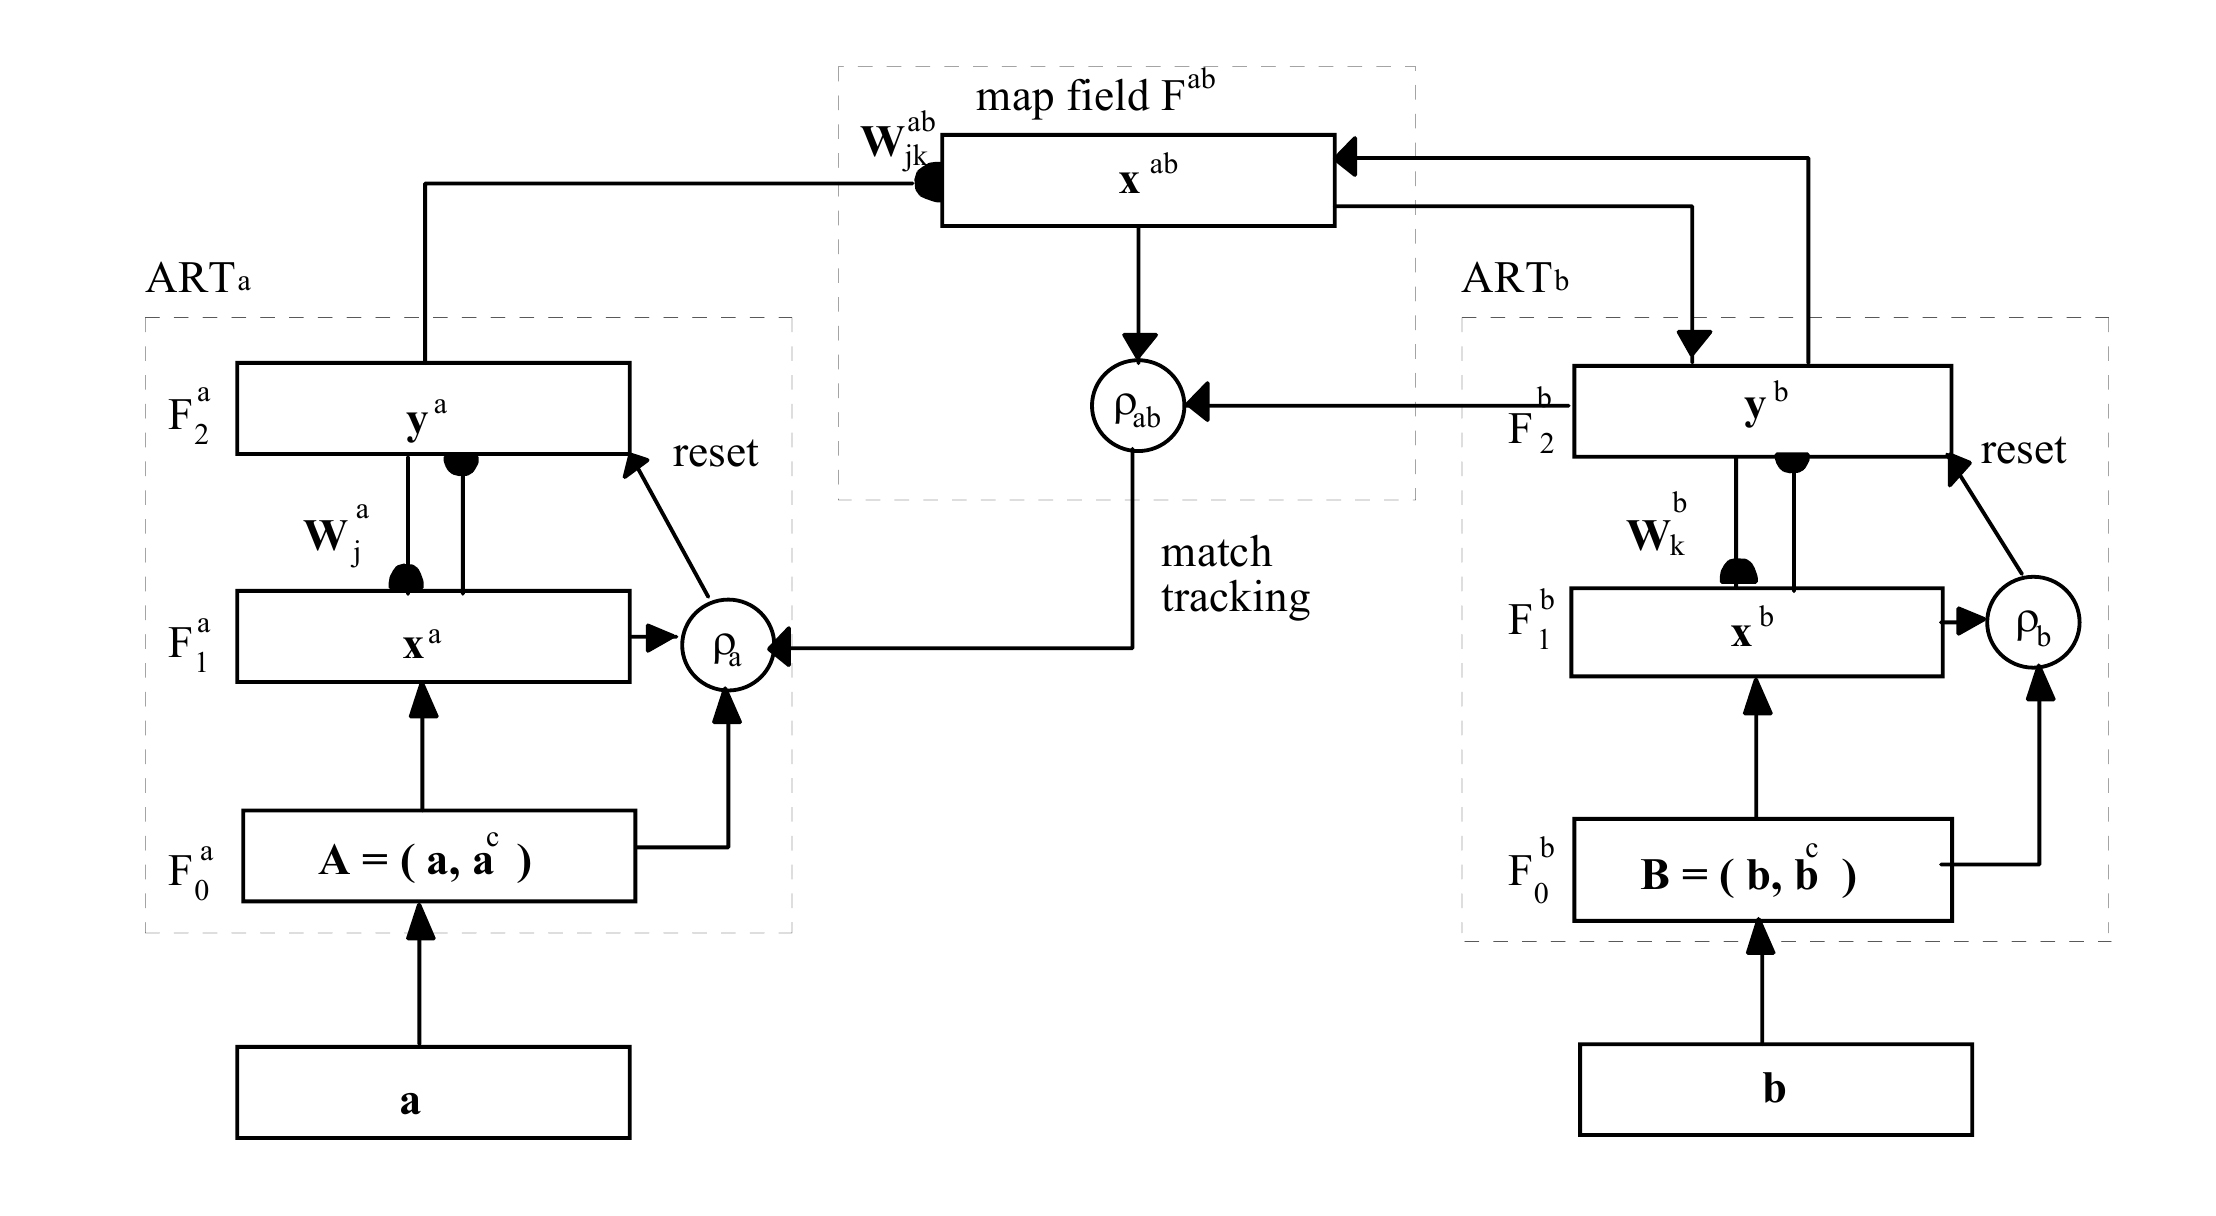
\includegraphics[width=14cm]{image_for_report/scheme.jpg}
\end{center}




\subsection{Состав и описание ПМО}

Программно-математическое обеспечение разрабатывалось в среде математического программирования Matlab.

ПМО включает следующие функции:
\begin{itemize}
	\item ARTMAP_Add_New_Category - добавление новой категории(класса) в сеть;
	\item ARTMAP_Classify - распознает образец на основе уже обученной сети;
	\item ARTMAP_Create_Network - создает новую сеть;
	\item ARTMAP_Learn - обучает сеть на заданной эталонной выборке;
	\item ART_Activate_Categories - вычисление значений активации для каждого образца;
	\item ART_Calculate_Match - вычисление степени соответствия;
	\item ART_Complement_Code - выполняет дополнительное кодирование над входными данными;
	\item ART_Update_Weights - обновляет веса для победившего класса.
\end{itemize}

ARTMAP_Example - содержит пример использования сети Fuzzy ARTMAP, используя вышеперечисленные функции, в нем непосредственно используются функции: RT_Complement_Code, ARTMAP_Create_Network, ARTMAP_Learn, ARTMAP_Classify.



\subsection{Тестирование ПМО}


Входными данными для обучения является изображение символов русского алфавита шириной 32 пикселя и высотой 32$\times$N пикселей, где N -количество символов в обучающей выборке (т.е. на один символ отводится $32\times 32$ пикселя). Для тестирования в графическом редакторе было создано изображение с 5 буквами (А, Б, В, Г, Д):
\begin{center}
	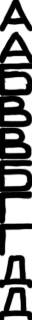
\includegraphics[width=10cm]{image_for_report/teach_5.jpg}
\end{center}

Порядок следования не важен, т.к. еще одним входным параметром является вектор значений названий классов соответственно в порядке их следования на изображении (в данном случае: {А,А,Б,В,В,Б,Г,Г,Д,Д}).

Далее изображение усредняется в области квадрата $2\times 2$ пикселя, т.о. на каждый символ теперь отводится $8\times 8$ пикселей. Получается такой результат
\begin{center}
	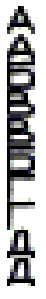
\includegraphics[width=10cm]{image_for_report/teach_5_2.jpg}
\end{center}

Это позволяет снизить временно-вычислительную сложность, оставив при этом достаточное количество элементов в векторе признаков каждого класса: $8 \cdot 8 = 64$.

После обучения сети на вход в функцию классификации подается изображение $32\times 32$ пикселя с распознаваемым символом. Он также проходит предварительную обработку по уменьшению разрешения.

Примеры распознавания:

Верно распознаются деформированные символы:
\begin{center}
	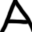
\includegraphics[width=5cm]{image_for_report/sample_a.bmp}
\end{center}
\begin{center}
	
\includegraphics[width=5cm]{image_for_report/sample_b_2.bmp}
\end{center}

Искаженные:
\begin{center}
	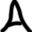
\includegraphics[width=5cm]{image_for_report/sample_a_2.bmp}
\end{center}

\begin{center}
	
\includegraphics[width=5cm]{image_for_report/sample_v_2.bmp}
\end{center}

\begin{center}
	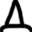
\includegraphics[width=5cm]{image_for_report/sample_d.bmp}
\end{center}

\begin{center}
	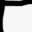
\includegraphics[width=5cm]{image_for_report/sample_g.bmp}
\end{center}

Смещенные с деформациями:
\begin{center}
	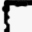
\includegraphics[width=5cm]{image_for_report/sample_g_2.bmp}
\end{center}

Однако, иногда, возникают случаи неверного распознавания, например:
\begin{center}
	
\includegraphics[width=5cm]{image_for_report/sample_v.bmp}
\end{center}
распозналось как Б.


При попытке распознать букву неизвестного пока класса, например:
\begin{center}
	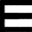
\includegraphics[width=5cm]{image_for_report/sample_e.bmp}
\end{center}
система в качестве результата классификации выдаст -1, при выполнив дообучение, после чего можно распознать изображение той же буквы:
\begin{center}
	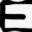
\includegraphics[width=5cm]{image_for_report/sample_e_2.bmp}
\end{center}
получив верный результат.




\subsection{Анализ результатов}

В результате работы с искуственной нейронной сетью Fuzzy ARTMAP можно отметить очевидные свойства ее применения:
\begin{itemize} \compact
 	\item параллельная классификация множества объектов, что потенциально позволяет использовать параллельные вычисления и получить высокую скорость обработки информации;
 	\item переобучение при успешной классификации, что позволяет иметь небольшое количество эталонов для обучения;
 	\item дополнительное обучение новым категориям в случае не соответствия распознаваемого объекта ни одному имеющемуся в "памяти" сети.
\end{itemize} 

Одновременно с этим переобучение при достаточно долгой эксплуатации может привести к вырождению классов, ввиду того, что при обучении используются операции выбора минимального значения признака. Это однако, можно предотвратить, либо периодической загрузкой эталонов, либо не использовать переобучении при наличии большого числа репрезентативных эталонов.


